\documentclass[11pt, twocolumn, twoside]{article}

\usepackage{graphicx}
\usepackage{amsmath, amssymb}
\usepackage{enumerate}
\usepackage{titleps}
\usepackage[top=1.25in,bottom=1in,right=0.75in,left=0.75in]{geometry}
\usepackage[parfill]{parskip}
\usepackage{titling}
\usepackage{hyperref}

\graphicspath{ {../images/} }

\newpagestyle{ruled}
{\setfoot{}{\thepage}{} \footrule}
\pagestyle{ruled}


\setlength{\droptitle}{-4em}   % This is your set screw
\posttitle{\par\end{center}\vskip 0.5em}


\title{6.867 Final Project Writeup} % Please change this
\date{}
\author {Vickie Ye and Alexandr Wang}


\begin{document}
\maketitle


\begin{abstract}
In this project, we compared different methods for facial expression recognition
using images from a Kaggle dataset released as a part of an ICML-2013 workshop
on representation learning.
We found that classification using features extracted manually from facial images
using principal component analysis yielded on average 40\% classification accuracy.
Using features extracted by facial landmark detection, we received on average 52\%
classification accuracy. However, when we used a convolutional neural network, we
received 65\% classification accuracy.
\end{abstract}

\section{Introduction}

In this project, we compared classification using features manually extracted from
facial images against classification using a convolutional neural net, which learns
the significant features of images through convolutional and pooling neural layers.
The two manual feature extraction methods we explored were principal component
analysis (PCA) and facial landmark detection. These extracted features were then
classified using a kernel support vector machine (SVM) and a neural network.

\subsection{PCA}

In facial recognition, PCA is used in generating a low-dimensional representation of
face images as linear combinations of the first $k$ eigenfaces of training data.
Eigenfaces are the eigenvectors of the training data's covariance matrix; the first
eigenfaces are the vectors along which the training data shows the highest variance.
Thus, we can express a facial image vector of thousands of pixels in terms of
the linearly independent basis of the first $k$ eigenvectors. 

\subsection{Facial Landmark Detection}

Facial landmarks can be extracted from facial images into lower-dimensional feature
vectors. The implementation that is used in this project uses the approach described
in \cite{Kazemi}. Kazemi et. al. uses localized histograms of gradient orientation in
a cascade of regressors that minimize squared error, in which each regressor is learned
through gradient boosting. This approach is robust to geometric and photometric
transformations, and showed less than 5\% error on the LFPW dataset.

The facial landmarks (eyes, eyebrows, nose, mouth) are intuitively the most expressive 
features in a face, and could also serve as good features for emotion classification.

\subsection{Kernel SVM}

Kernel SVM is 

\subsection{Neural Network}

An artificial neural network uses

\subsection{Convolutional Neural Networks}

Convolutional neural networks (CNNs) are artificial neural networks that work particularly well for image data. The structure of CNNs exploits strong local correlation in the inputs. This is done by enforcing local connectivity between neurons of adjacent layers. The inputs of a hidden unit at a particular layer $n$ are some locally-connected subset of the units of the previous layer $n-1$, done in such a way that the input to layer $n$ represent some tile of the units of layer $n-1$, where all the tiles overlap.

In addition, CNNs utilize shared parameterizations (weight vector and bias) across layers. By constraining the same types of weights across layers, essentially replicating units across layers, allows for features to be detected regardless to their position in the initial input, making the network much more robust to real world image data. Additionally, by constraining multiple weights to be the same reduces the parameters to be learnt, increasing learning efficiency.

\section{Experimental Details}

\subsection{Datasets}

For this project, we primarily used a dataset released by Kaggle as a part of an
ICML-2013 workshop in representation learning. This dataset included 28,709 labeled
training images, and two labeled test sets of 3,589 images. We also used images from
........

\subsection{PCA}
We used \texttt{sklearn}'s implementation of PCA to extract eigenfaces from our data.

\begin{figure}
\centering
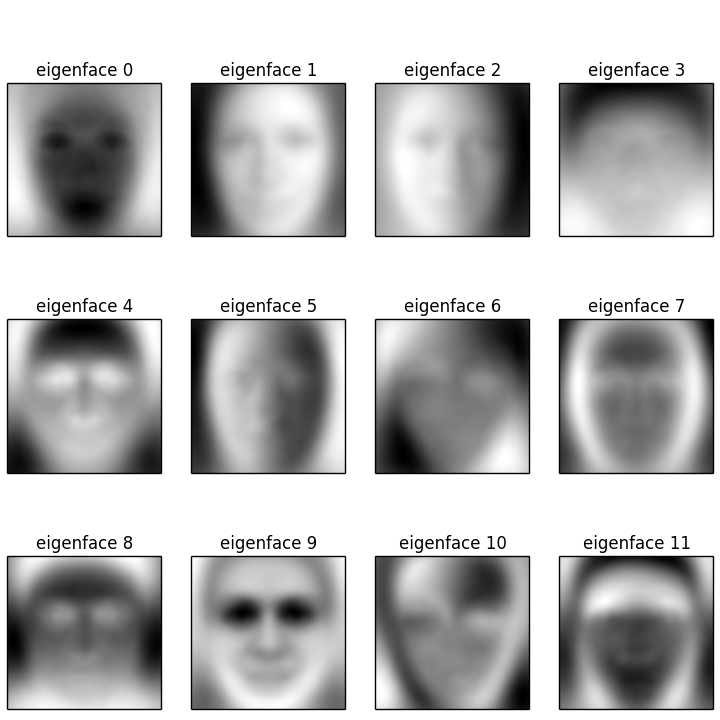
\includegraphics[width=\textwidth]{eigenfaces}
\caption{\label{fig:eigenfaces} The first 12 eigenfaces generated through PCA from the
training data.}
\end{figure}

\subsection{Facial Landmarks}


\begin{figure}
\centering
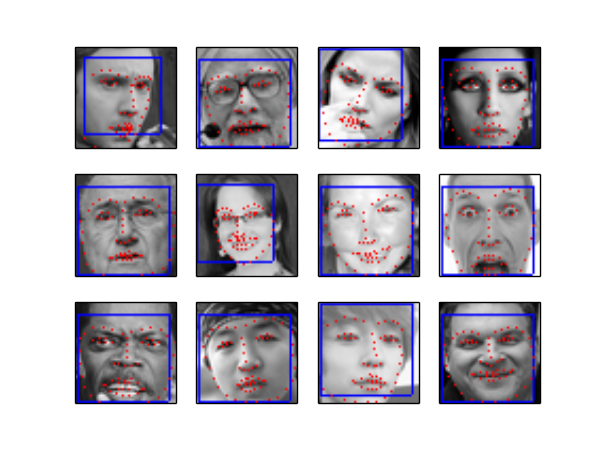
\includegraphics[width=\textwidth]{landmarks}
\caption{\label{fig:landmarks} The first 12 test images with labeled facial landmarks
as generated from DLib's shape recognizer.}
\end{figure}

\subsection{Kernel Support Vector Machine}

\subsection{Neural Network}

\subsection{Convolutional Neural Network}

To implement our convolutional neural network, we used Google's TensorFlow neural network library.
Our model follows the architecture described in \cite{Krizhevsky}, with a few differences in the top few layers.
In particular, we use fully connected layers instead of locally connected layers. The model described in
\cite{Krizhevsky} was designed for ImageNet's object classification, but it translated well to our problem of classifying facial expressions.

\subsubsection{Network Structure}

\begin{figure}
	\centering
	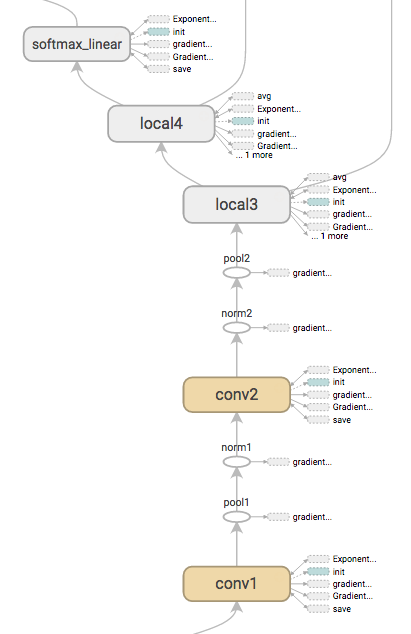
\includegraphics[width=3.25in]{inference_graph}
	\caption{TensorFlow computation graph for the neural network in the CNN we implemented, illustrating each of the layers and computation done in between each layer.}
	\label{fig:inference}
\end{figure}

We implemented a deep CNN with five layers, which are from front to back: \texttt{conv1}, \texttt{conv2}, \texttt{local3}, \texttt{local4}, and \texttt{softmax\_linear}. This structure is illustrated in Figure \ref{fig:inference}. 

The layers \texttt{conv1} and \texttt{conv2} are convolution layers, which divides the image into overlapping tiles and use those as inputs to the next layer. In detail, the expression is
\[ y(i, j) = \sum_{di, dj} x(s_1i + di, s_2j + dj) f(di, dj)\]
where $y(\cdot, \cdot)$ is the output, $di$ and $dj$ are changes which range over the tile size, $s_1$ and $s_2$ are strides which measure how much you move between each convolution window across each dimension, $x(\cdot, \cdot)$ is the input, and $f(\cdot, \cdot)$ are filters, which are the weights for the layer. We didn't employ any regularization on these convolution layers, and we used window sizes of 5 by 5 pixels with a strides of 1.

As illustrated in Figure \ref{fig:inference}, after each convolution layer, we performed a \texttt{pool1} operation and a \texttt{norm1} operation. The \texttt{pool1} operation is max pooling, which will transform the input to take the maxima in tiles similarly to the convolution step. In detail,
\[ y(i, j) = \max_{di, dj} x(s_1i + di, s_2j + dj)\]
with each term defined as before. Note that this is not a layer because there are no weights. The \texttt{norm1} operation is a local response normalization response, where each input is normalized by dividing it by the squared sum of inputs within a certain radius of it. This technique is described in more detail in \cite{Krizhevsky}, and serves as form of ``brightness normalization" on the input.

The \texttt{local3} and \texttt{local4} are fully connected layers with rectified linear activation according to $f(x) = \max(x, 0)$. We employ regularization on both of these errors by adding the L2-loss of weights on both layers to our total loss function. 

Finally, the \texttt{softmax\_linear} layer is linear transformation layer that produces logits according to a simple linear transformation based on learned weights and biases.

\subsubsection{Training}

The loss function we minimized was primarily the cross entropy between the multinomial distribution, formed by the normalized logits outputted by our CNN, and the probability distribution that is 1 for the correct class and 0 for all other classes. The expression for cross entropy between two probability distributions $p, q$ is
\[H(p, q) = E_p[-\log q] = -\sum_x p(x)\log q(x)\]
which measures the divergence between the two discrete probability distributions. In addition, we added standard weight decay, i.e. L2-loss, for the weights of the \texttt{local3} and \texttt{local4} layers for weight regularization.

For training, we fed the model randomly distorted training examples (see subsection \ref{overfitting}) in randomly shuffled batches of 128 samples each. For each of these examples, we would determine our loss based on our current inference. After each batch, we performed back propagation using gradient descent to learn the weights, and we called each time we finished a batch a step.


\subsubsection{Minimizing Overfitting} \label{overfitting}

Since the size of our training set was 28,709 labeled examples, and our neural net needed to go through many more than 28,000 examples to achieve convergence, we employed a few techniques to ensure that our convolutional neural net did not overfit to the training set.

First off, we implemented learning rate decay on our convolutional neural net, so that the learning rate decreased as it had been trained through more examples. We used exponential decay, so that that the learning rate decayed by a factor of $0.1$ after training through $1,200,000$ examples, and we had it decay in a step change manner as is visible in Figure \ref{fig:cnnloss}. We found that the step change learning rate decay worked better than a continuous exponential decay. This could be because maintaining a high learning rate initially could ensure that the CNN was trained towards a good local optimum in fewer steps, whereas a steadily decreasing learning rate could limit the range of the neural network.

In addition, we implemented distortion of the images while training to artificially increase the size of our training set, and make our convolutional neural net more robust to slightly distorted inputs. We processed our images in a few different ways. We would crop our 48 by 48 pixel images to a 40 by 40 pixel box, centrally for model evaluation and randomly for training. Then we approximately whiten the photos, scaling the pixel values linearly so that they pixel values have a mean of 0 and a standard deviation of 1, essentially normalizing them. This ensures consistent inputs to our neural network.

For training in particular, we would do a few more distortions to artificially increase our training set. We randomly flipped the image from left to right, randomly distorted the image brightness, and 	randomly distorted the image contrast for each image. These changes to randomly distort the images greatly improved the performance of the model, raising the correct classification rate from $45.4\%$ to $53.8\%$ when initially implemented.

\section{Results and Analysis}

\subsection{Facial Landmarks}

\subsection{Convolutional Neural Network}

\begin{figure}
	\centering
	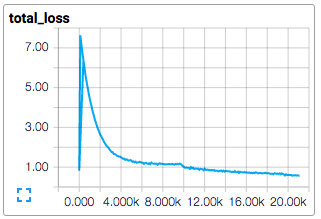
\includegraphics[width=3in]{total_loss}
	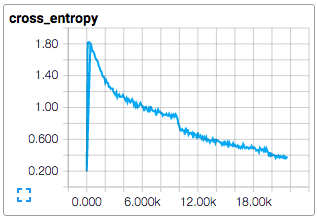
\includegraphics[width=3in]{cross_entropy}
	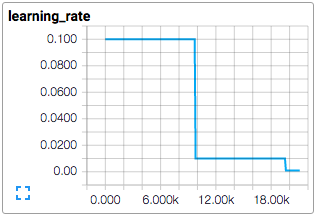
\includegraphics[width=3in]{learning_rate}
	\caption{The total loss, cross entropy, and learning rate of the convolutional neural net over time.}
	\label{fig:cnnloss}
\end{figure}

\begin{figure}
	\centering
	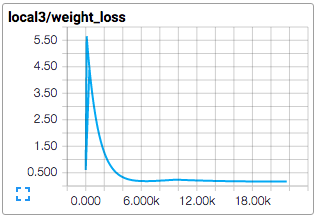
\includegraphics[width=3in]{local3_loss}
	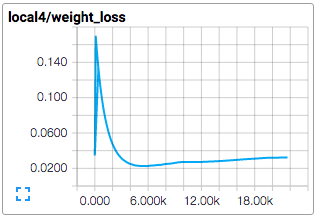
\includegraphics[width=3in]{local4_loss}
	\caption{The loss on the local3 layer and local4 layer over time in the convolutional neural net.}
	\label{fig:layer_loss}
\end{figure}

\subsection{Comparison between the two}


\begin{thebibliography}{9}
\bibitem{Lawrence}
Lawrence, S.; Giles, L.; Tsoi, A. C.; Back, A. D. (1997)
``Face Recognition: A Convolutional Neural-Network Approach"
\textit{Neural Networks, IEEE transactions on} 8 (1):98-113
\bibitem{Matsugu}
Matsugu, M.; Mori, K.; Mitari Y.; Kaneda Y. (2003)
``Subject independent facial expression recognition with robust face detection using a convolutional neural network"
\textit{Neural Networks} 16 (5):555-559


\bibitem{Krizhevsky}
Krizhevsky, A.; Sutskever; Hinton, I.; Hinton, G. (2012)
``ImageNet Classification with Deep Convolutional Neural Networks"
\textit{Advances in Neural Information Processing Systems} 25 (1):1097-1105
\end{thebibliography}


\end{document}
